\documentclass[10pt]{article}
\usepackage[a4paper,margin=2.5cm]{geometry}
\usepackage{lmodern}
\usepackage{amsmath,amssymb}
\usepackage{booktabs}
\usepackage{tabularx}
\usepackage{ltablex}
\keepXColumns
\usepackage{enumitem}
\usepackage{caption}
\usepackage{parskip}
\usepackage{tikz}
\usetikzlibrary{positioning}

\usepackage[colorlinks=true, linkcolor=blue, citecolor=blue, urlcolor=blue]{hyperref}
\usepackage{xurl}

\renewcommand{\arraystretch}{1.2}
\captionsetup{hypcap=false}

\title{\textbf{Aquablend --- MILP Mathematical Formulation}}
\author{MILP Stream}
\date{}

\begin{document}
\maketitle

\section{Overview}

Water corporations draw drinking water from multiple sources, such as reservoirs, river intakes, and groundwater bores, that differ in cost and in raw water quality (pH, alkalinity, turbidity, and so on).
Before that water can be supplied for human consumption, it is treated at a plant and delivered to demand zones.
The question this model answers is:
which sources should be drawn from, how much from each, and how should that water be routed to plants and zones, so that demand is met, and water quality stays within safe limits, at the lowest possible cost?

This is formulated as a Mixed-Integer Linear Program (MILP).
Whether a source, plant, or transfer link is used at all is a binary decision; how much water is drawn or flows along each link is a continuous decision.
The objective balances fixed activation costs against the variable cost of drawing, transferring and treating water.

Treatment is modelled in three parts.
A flat rate per megalitre (ML) covers the cost of operating a plant, each removal process is charged based on the load it removes, and chemical dosing is charged based on the mass of chemical used.
The load-based removal cost and chemical dosing cost make source blending an economic decision rather than purely a feasibility problem:
a cheaper but more contaminated source may incur higher treatment costs than a cleaner, more expensive source.
Removal processes reduce parameter loads, while chemical dosing can add load for supported quality parameters where a defensible linear conversion is available.
This allows the model to represent both removal of excessive constituents and chemical adjustment used to meet required lower quality limits.

The toy case considers the simplest version of this problem:
one treatment plant and one demand zone, fed by several candidate sources.
With only one plant and one zone, there is no routing choice to make:
every active source sends its full withdrawal to the plant, and the plant sends its entire outflow to the demand zone.
As a result, the routing variables are determined by the source withdrawals, leaving the model to determine which sources to activate, how much to draw from each, and any required treatment decisions.
Section~\ref{sec:toy} derives this toy case as a special case of the general network formulation, so the same formulation can later be extended to multiple plants and zones without being rebuilt from scratch.

\section{Notation}

\paragraph{Convention.}
This is a single-period model (one representative day), so no day index is used.
Parameters are uppercase; decision variables are lowercase, using Greek letters for binary decisions and lowercase Latin for continuous quantities.
A subscript is an index; an overbar/underbar is an upper/lower bound.

\subsection{Sets}

\begin{tabularx}{\textwidth}{@{}lX@{}}
    % You can change the table name if you'd like, since I see later you mention Table 1, 
    % but I'm afraid they could not find ``Table 1''.
    \caption{Notations on sets of input parameters}
    \label{tab:sets}                                                             \\
    \toprule
    \textbf{Notation} & \textbf{Description}                                     \\
    \midrule
    \endfirsthead

    \toprule
    \textbf{Notation} & \textbf{Description}                                     \\
    \midrule
    \endhead

    \midrule
    \multicolumn{2}{r}{\emph{Continued on next page}}                            \\
    \endfoot
    \bottomrule
    \endlastfoot
    $\mathcal{S}$     & set of water sources, $s \in \mathcal{S}$                \\
    $\mathcal{T}$     & set of treatment plants, $t \in \mathcal{T}$             \\
    $\mathcal{Z}$     & set of demand zones, $z \in \mathcal{Z}$                 \\
    $\mathcal{P}$     & set of water quality parameters, $p \in \mathcal{P}$     \\
    $\mathcal{R}$     & set of removal processes, $r \in \mathcal{R}$            \\
    $\mathcal{R}_t$   & processes installed at plant $t$, as an ordered sequence
    $r_1, \dots, r_{n_t}$ drawn from $\mathcal{R}$, in the order water
    flows through them                                                           \\
    $\mathcal{K}$     & set of treatment chemicals and additives, $c \in \mathcal{K}$ \\
    $\mathcal{K}_t$   & subset of treatment chemicals and additives available for dosing at plant $t$, with $\mathcal{K}_t \subseteq \mathcal{K}$ \\
\end{tabularx}
$n_t = |\mathcal{R}_t|$ is written with the index because plants differ in how many processes they run.
For example, a plant with coagulation, filtration and chlorination has $n_t = 3$, while one with filtration alone has $n_t = 1$.

The plant specific set $\mathcal{K}_t$ represents chemical availability at plant $t$.
Unlike $\mathcal{R}_t$, which is ordered to represent the treatment sequence, $\mathcal{K}_t$ is an unordered subset containing only the chemicals and additives that can be dosed at plant $t$.

\subsection{Parameters}
\begin{tabularx}{\textwidth}{@{}lXl@{}}
    % Same reason.
    \caption{Notations on input parameters}
    \label{tab:parameters}                                                                                                                                  \\
    \toprule
    \textbf{Notation}    & \textbf{Description}                                                                                  & \textbf{Units}           \\
    \midrule
    \endfirsthead

    \toprule
    \textbf{Notation}    & \textbf{Description}                                                                                  & \textbf{Units}           \\
    \midrule
    \endhead

    \midrule
    \multicolumn{3}{r}{\emph{Continued on next page}}                                                                                                       \\
    \endfoot

    \bottomrule
    \endlastfoot

    \multicolumn{3}{@{}l}{\emph{Demand}}                                                                                                                    \\
    $D_{z}$              & volume of water to deliver to demand zone $z$                                                         & ML/day                   \\[0.4em]
    \midrule
    \multicolumn{3}{@{}l}{\emph{Sources}}                                                                                                                   \\

    $F_{s}$              & fixed cost of activating source $s$                                                                   & \$/day                   \\
    $C_{s}$              & unit cost of drawing water from source $s$                                                            & \$/ML                    \\
    $\underline{W}_{s}$  & minimum daily withdrawal from source $s$                                                              & ML/day                   \\
    $\overline{W}_{s}$   & maximum daily withdrawal from source $s$                                                              & ML/day                   \\[0.4em]
    \midrule
    \multicolumn{3}{@{}l}{\emph{Treatment plants}}                                                                                                          \\
    $F_{t}$              & fixed cost of activating treatment plant $t$                                                          & \$/day                   \\

    $C_{t}$              & unit treatment cost at plant $t$                                                                      & \$/ML                    \\
    $\underline{V}_{t}$  & minimum daily throughput of plant $t$                                                                 & ML/day                   \\
    $\overline{V}_{t}$   & maximum daily throughput of plant $t$                                                                 & ML/day                   \\[0.4em]
    \midrule
    \multicolumn{3}{@{}l}{\emph{Arcs}}                                                                                                                      \\
    $\overline{L}_{st}$  & maximum flow on the arc from source $s$ to plant $t$                                                  & ML/day                   \\
    $\overline{L}_{tz}$  & maximum flow on the arc from plant $t$ to zone $z$                                                    & ML/day                   \\
    $C_{st}$             & unit cost of transferring water from source $s$ to plant $t$                                          & \$/ML                    \\
    $C_{tz}$             & unit cost of transferring water from plant $t$ to zone $z$                                            & \$/ML                    \\[0.4em]
    \midrule
    \multicolumn{3}{@{}l}{\emph{Water quality}}                                                                                                             \\
    $Q_{sp}$             & value of quality parameter $p$ in source $s$                                                          & units of $p$             \\
    $\underline{Q}_{p}$  & lower regulatory limit for parameter $p$                                                              & units of $p$             \\
    $\overline{Q}_{p}$   & upper regulatory limit for parameter $p$                                                              & units of $p$             \\
    $\underline{I}_{tp}$ & minimum value of $p$ that plant $t$ can accept                                                        & units of $p$             \\
    $\overline{I}_{tp}$  & maximum value of $p$ that plant $t$ can accept                                                        & units of $p$             \\[0.4em]
    \midrule
    \multicolumn{3}{@{}l}{\emph{Removal processes}}                                                                                                         \\
    $F_{tr}$             & fixed daily cost of operating process $r$ at plant $t$                                                & \$/day                   \\
    $C_{trp}$            & cost per unit of load of $p$ removed by process $r$ at plant $t$                                      & \$/(units of $p\cdot$ML) \\
    $H_{trp}$            & maximum fraction of the load of $p$ removable by process $r$ at plant $t$, with $0 \le H_{trp} \le 1$ & ---                      \\[0.4em]
    \midrule
    \multicolumn{3}{@{}l}{\emph{Chemical dosing}}                                                                                                             \\
    $C^{\mathrm{chem}}_{tc}$ & unit purchase cost of chemical $c$ at plant $t$                                                    & \$/kg                    \\
    $\underline{\rho}_{tc}$ & minimum dose rate when chemical $c$ is active at plant $t$                                         & mg/L                     \\
    $\overline{\rho}_{tc}$  & maximum dose rate of chemical $c$ at plant $t$                                                       & mg/L                     \\
    $\eta_{cp}$          & contribution of quality parameter $p$ per unit mass of chemical $c$                                    & $((\text{units of }p)\cdot\text{ML})/\text{kg}$ \\
\end{tabularx}
The plant specific chemical parameters $C^{\mathrm{chem}}_{tc}$, $\underline{\rho}_{tc}$ and $\overline{\rho}_{tc}$ are defined only for $c \in \mathcal{K}_t$.
The coefficient $\eta_{cp}$ is defined for chemical quality pairs $c \in \mathcal{K}$ and $p \in \mathcal{P}$; unsupported linear relationships are represented by setting $\eta_{cp}=0$.

Costs and limits are treated as fixed.
The units of a quality parameter depend on $p$ (e.g.\ mg/L, NTU).
Quality parameters that are not approximately linear in their natural units are represented using transformed quantities chosen to support linear blending within the MILP.
For $p=\mathrm{pH}$, the MILP uses scaled hydrogen ion concentration in nmol/L rather than raw pH units; the source values and corresponding inlet and regulatory bounds are all represented on this same scale.

The inlet limits $\underline{I}_{tp}$ and $\overline{I}_{tp}$ bound the same physical quantity as the regulatory limits $\underline{Q}_{p}$ and $\overline{Q}_{p}$, but they have different meanings.
$I$ is what a plant can accept, while $Q$ denotes the standards that the water must meet after treatment before reaching the demand zone.

$C_{trp}$ is charged per unit of load removed.
When $p$ is represented as a concentration, multiplying concentration by volume gives a quantity proportional to mass, subject to consistent units.
For parameters such as turbidity measured in NTU, the cost is per NTU$\cdot$ML, which is not a mass; however, we assume it correlates to the mass of sediment that would produce that level of turbidity.

For chemical dosing, $\underline{\rho}_{tc}$ and $\overline{\rho}_{tc}$ are concentration based operating bounds, while the optimisation variable introduced below is the total chemical mass used per day.
The coefficient $\eta_{cp}$ converts chemical mass into the same load units used by the water quality formulation.
When chemical $c$ has no supported linear effect on parameter $p$, $\eta_{cp}$ is set to zero.
In the initial MILP, this includes direct pH adjustment, which is not represented by a constant linear chemical effect coefficient.

\subsection{Decision variables}
\begin{tabularx}{\textwidth}{@{}llll@{}}
    % Same reason.
    \caption{Notations on decision variables}
    \label{tab:variables}                                                                                                                       \\
    \toprule
    \textbf{Notation} & \textbf{Domain}             & \textbf{Description}                                        & \textbf{Units}              \\
    \midrule
    \endfirsthead

    \toprule
    \textbf{Notation} & \textbf{Domain}             & \textbf{Description}                                        & \textbf{Units}              \\
    \midrule
    \endhead

    \midrule
    \multicolumn{4}{r}{\emph{Continued on next page}}                                                                                           \\
    \endfoot

    \bottomrule
    \endlastfoot

    \multicolumn{4}{@{}l}{\emph{Sources}}                                                                                                       \\
    $\alpha_{s}$      & $\{0,1\}$                   & $1$ if source $s$ is activated                              & ---                         \\
    $a_{s}$           & $\ge 0$                     & volume drawn from source $s$                                & ML/day                      \\[0.4em]
    \midrule
    \multicolumn{4}{@{}l}{\emph{Treatment plants}}                                                                                              \\
    $\beta_{t}$       & $\{0,1\}$                   & $1$ if plant $t$ is activated                               & ---                         \\[0.4em]
    \midrule
    \multicolumn{4}{@{}l}{\emph{Arcs}}                                                                                                          \\
    $\gamma_{st}$     & $\{0,1\}$                   & $1$ if source $s$ sends water to plant $t$                  & ---                         \\
    $b_{st}$          & $\ge 0$                     & volume of water from source $s$ to plant $t$                & ML/day                      \\
    $\delta_{tz}$     & $\{0,1\}$                   & $1$ if plant $t$ sends water to demand zone $z$             & ---                         \\
    $c_{tz}$          & $\ge 0$                     & volume of water from plant $t$ to demand zone $z$           & ML/day                      \\[0.4em]
    \midrule
    \multicolumn{4}{@{}l}{\emph{Removal processes}}                                                                                             \\
    $\sigma_{tr}$     & $\{0,1\}$                   & $1$ if removal process $r$ is operated at plant $t$         & ---                         \\
    $e_{trp}$         & $\ge 0$                     & load of parameter $p$ removed by process $r$ at plant $t$   & (units of $p$)$\cdot$ML/day \\
    $\ell^i_{tp}$     & $\ge 0$                     & load of $p$ remaining after the $i$-th process at plant $t$
                      & (units of $p$)$\cdot$ML/day                                                                                             \\[0.4em]
    \midrule
    \multicolumn{4}{@{}l}{\emph{Chemical dosing}}                                                                                              \\
    $\kappa_{tc}$      & $\{0,1\}$                   & $1$ if chemical $c$ is actively dosed at plant $t$                   & ---                         \\
    $m_{tc}$            & $\ge 0$                      & mass of chemical $c$ dosed at plant $t$                             & kg/day                      \\
\end{tabularx}
$\sigma_{tr}$ and $e_{trp}$ are defined only for $r \in \mathcal{R}_t$, and
$\ell^i_{tp}$ only for $i = 0, \dots, n_t$; the objective and constraints below reflect this.
Since we have $\mathcal{R}_t = (r_1, \dots, r_{n_t})$ (Table~\ref{tab:sets}), the process at stage $i$ is $r_i$:
variables are indexed by the process itself, so $e_{t r_i p}$ is the same variable as $e_{trp}$ with $r = r_i$.

Likewise, the chemical variables $\kappa_{tc}$ and $m_{tc}$ are defined only for $c \in \mathcal{K}_t$.
This avoids introducing chemical decision variables for chemicals that are not available at plant $t$.

The chemical mass variable $m_{tc}$ is used instead of dose concentration as the primary optimisation variable.
This keeps chemical cost and quality load additions linear.
The corresponding dose rate in mg/L is recovered after optimisation from the solved chemical mass and plant throughput.

\section{Example network structure}
\begin{center}
    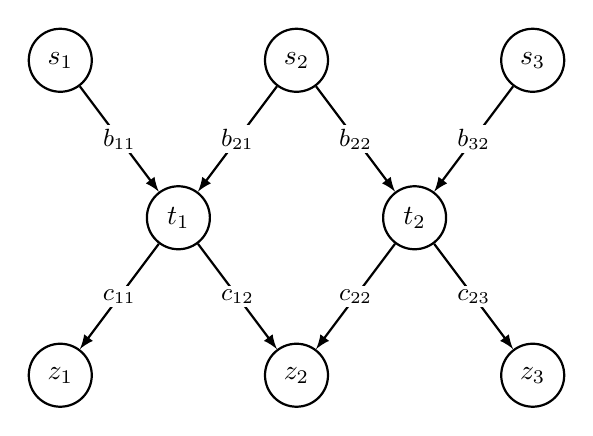
\begin{tikzpicture}[
            nd/.style={circle, draw, minimum size=8mm, inner sep=1pt},
            every edge/.style={draw, -latex, thick},
            lbl/.style={fill=white, inner sep=1.5pt, font=\small},
            thick
        ]
        % Source nodes
        \node[nd] (S1) at (0,4)   {$s_1$};
        \node[nd] (S2) at (3,4)   {$s_2$};
        \node[nd] (S3) at (6,4)   {$s_3$};

        % Treatment plant nodes
        \node[nd] (T1) at (1.5,2) {$t_1$};
        \node[nd] (T2) at (4.5,2) {$t_2$};

        % Demand zone nodes
        \node[nd] (Z1) at (0,0)           {$z_1$};
        \node[nd] (Z2) at (3,0)           {$z_2$};
        \node[nd] (Z3) at (6,0)           {$z_3$};

        % S -> T connections
        \draw (S1) edge node[lbl] {$b_{11}$} (T1);
        \draw (S2) edge node[lbl] {$b_{21}$} (T1);
        \draw (S2) edge node[lbl] {$b_{22}$} (T2);
        \draw (S3) edge node[lbl] {$b_{32}$} (T2);

        % T -> Z connections
        \draw (T1) edge node[lbl] {$c_{11}$} (Z1);
        \draw (T1) edge node[lbl] {$c_{12}$} (Z2);
        \draw (T2) edge node[lbl] {$c_{22}$} (Z2);
        \draw (T2) edge node[lbl] {$c_{23}$} (Z3);
    \end{tikzpicture}
    \captionof{figure}{One example of the network structure (sources $\to$ treatment plants $\to$ demand zones).
        Each source-plant arc has an activation binary $\gamma_{st}$ and a flow variable $b_{st}$; each plant-zone arc has $\delta_{tz}$ and $c_{tz}$.
        The formulation is generic over any number of sources, plants, zones and links.
    }
\end{center}

\section{Objective}
Minimise total cost over a single period.

Costs are grouped according to the part of the network to which they belong:
sources, arcs, plants, removal processes, and chemical dosing.
Sources and plants carry fixed activation costs and variable costs based on the volume handled.
Removal processes carry a fixed operating cost and a variable cost based on the load removed.
Chemical dosing is charged according to the mass of each chemical used, reflecting the economic trade-off between treatment performance and chemical consumption \cite{Li2022CoagulantDose}.
Arcs are charged on flow volume only, since the model does not currently assign a fixed cost to activating a link.

The removal and chemical costs make source blending an economic decision rather than purely a feasibility problem.
A source requiring greater contaminant removal or additional chemical adjustment may incur a higher treatment cost than a source whose raw quality is naturally closer to the required outlet limits.
\begin{equation}
    \begin{aligned}
        \min \quad
                     & \sum_{s \in \mathcal{S}}
        F_s \alpha_s &                          & \text{source fixed cost} \\ + \; & \sum_{s \in \mathcal{S}} C_s a_s & & \text{source draw cost} \\ + \; & \sum_{t \in \mathcal{T}} F_t \beta_t & & \text{plant fixed cost} \\ + \; & \sum_{t \in \mathcal{T}} C_t \sum_{s \in \mathcal{S}} b_{st} & & \text{plant throughput cost} \\ + \; & \sum_{s \in \mathcal{S}} \sum_{t \in \mathcal{T}} C_{st}\, b_{st} + \sum_{t \in \mathcal{T}} \sum_{z \in \mathcal{Z}} C_{tz}\, c_{tz} & & \text{arc transfer cost} \\ + \; & \sum_{t \in \mathcal{T}} \sum_{r \in \mathcal{R}_t} F_{tr} \sigma_{tr} & & \text{removal process fixed cost} \\ + \; & \sum_{t \in \mathcal{T}} \sum_{r \in \mathcal{R}_t} \sum_{p \in \mathcal{P}} C_{trp}\, e_{trp} & & \text{removal cost} \\ + \; & \sum_{t \in \mathcal{T}} \sum_{c \in \mathcal{K}_t} C^{\mathrm{chem}}_{tc}\, m_{tc} & & \text{chemical dosing cost}
    \end{aligned}
\end{equation}


\section{Constraints}
\label{sec:constraints}
\paragraph{Non-negativity.}
All continuous variables must be non-negative.
\begin{equation}\label{eq:nonnegativity}
\begin{aligned}
    a_s &\ge 0,
    && \forall s \in \mathcal{S},\\
    b_{st} &\ge 0,
    && \forall s \in \mathcal{S},\ \forall t \in \mathcal{T},\\
    c_{tz} &\ge 0,
    && \forall t \in \mathcal{T},\ \forall z \in \mathcal{Z},\\
    e_{trp} &\ge 0,
    && \forall t \in \mathcal{T},\ \forall r \in \mathcal{R}_t,\ \forall p \in \mathcal{P},\\
    \ell^i_{tp} &\ge 0,
    && \forall t \in \mathcal{T},\ \forall p \in \mathcal{P},\ i = 0,\dots,n_t,\\
    m_{tc} &\ge 0,
    && \forall t \in \mathcal{T},\ \forall c \in \mathcal{K}_t.
\end{aligned}
\end{equation}

\paragraph{Demand satisfaction.}
The total volume of water sent from all treatment plants to demand zone $z$ via the arcs $c_{tz}$ must be at least the demand $D_z$ for that zone.
\begin{equation}
    \sum_{t \in \mathcal{T}} c_{tz} \ge D_z, \qquad \forall z \in \mathcal{Z}.
\end{equation}

\paragraph{Source capacity and activation.}
Water can only be drawn from a source if it has been activated.
If source $s$ is inactive ($\alpha_s = 0$), the draw $a_s$ is forced to zero.
If source $s$ is active ($\alpha_s = 1$), the draw must lie between its minimum daily withdrawal $\underline{W}_s$ and maximum daily withdrawal $\overline{W}_s$.
\begin{equation}\label{eq:source_capacity}
    \underline{W}_s\alpha_s
    \leq
    a_s
    \leq
    \overline{W}_s\alpha_s,
    \quad \forall s \in \mathcal{S}.
\end{equation}

\paragraph{Plant capacity and activation.}
A plant can process water only if it has been activated.
If plant $t$ is inactive ($\beta_t=0$), the total volume arriving from all sources is forced to zero.
If plant $t$ is active ($\beta_t=1$), the total incoming volume must lie between its minimum daily throughput $\underline{V}_t$ and maximum daily throughput $\overline{V}_t$.
\begin{equation}\label{eq:plant_capacity}
    \underline{V}_t \beta_t
    \leq
    \sum_{s \in \mathcal{S}} b_{st}
    \leq
    \overline{V}_t \beta_t,
    \quad \forall t \in \mathcal{T}.
\end{equation}

\paragraph{Plant flow conservation.}
The total volume leaving plant $t$ toward all zones via the arcs $c_{tz}$ equals the total volume entering it from all sources via the arcs $b_{st}$.
\begin{equation}
    \sum_{z \in \mathcal{Z}} c_{tz} = \sum_{s \in \mathcal{S}} b_{st},
    \quad \forall t \in \mathcal{T}.
\end{equation}

\paragraph{Source flow conservation.}
The volume drawn from each source $a_{s}$ must equal the total volume it sends to all plants via the arcs $b_{st}$.
\begin{equation}
    a_s = \sum_{t \in \mathcal{T}} b_{st} , \quad \forall s \in \mathcal{S}.
\end{equation}

\paragraph{Arc capacity.}
Each arc has a maximum flow and can carry water only if that arc is active.
For a source-to-plant arc, the flow $b_{st}$ is capped at $\overline{L}_{st}$ and forced to zero unless the arc is active ($\gamma_{st} = 1$).
\begin{equation}
    b_{st} \le \overline{L}_{st} \gamma_{st}, \quad \forall s \in \mathcal{S}, t \in \mathcal{T}.
\end{equation}
Similarly, a plant-to-zone arc's flow $c_{tz}$ is capped at $\overline{L}_{tz}$ and is zero unless the arc is active ($\delta_{tz} = 1$).
\begin{equation}
    c_{tz} \le \overline{L}_{tz} \delta_{tz}, \quad \forall t \in \mathcal{T}, z \in \mathcal{Z}.
\end{equation}

\paragraph{Arcs require active nodes.}
Arcs can only be active if the corresponding upstream node (source or treatment plant) is active.
This is enforced by ensuring that the binary variables representing the arcs are less than or equal to the binary variables representing the activation of the sources and plants.
A source-to-plant arc requires the source to be active:
\begin{equation}
    \gamma_{st} \le \alpha_s, \quad \forall s \in \mathcal{S}, t \in \mathcal{T}.
\end{equation}
A plant-to-zone arc requires the plant to be active:
\begin{equation}
    \delta_{tz} \le \beta_t,  \quad \forall t \in \mathcal{T}, z \in \mathcal{Z}.
\end{equation}
\emph{Optional}: a source-to-plant arc could also require the plant to be active,
\begin{equation}
    \gamma_{st} \le \beta_t, \quad \forall s \in \mathcal{S},\, t \in \mathcal{T}.
\end{equation}
This is not explicitly needed, since zero flow to an inactive plant is already guaranteed by the plant capacity constraint~\eqref{eq:plant_capacity}.
Suppose the plant $t$ is inactive, so $\beta_t = 0$.
Then~\eqref{eq:plant_capacity} becomes
\begin{equation*}
    \sum_{s \in \mathcal{S}} b_{st} \le \overline{V}_t\,\beta_t = 0,
\end{equation*}
and since every flow is non-negative ($b_{st} \ge 0$), this forces $b_{st} = 0$ for all $s \in \mathcal{S}$.

\paragraph{Inlet treatability.}
A plant can only accept raw water that its installed processes are built to handle.
This is a property of the plant rather than a regulatory standard, which is the reason the bound includes the index $t$.
\begin{equation}\label{eq:inlet_treatability}
    \underline{I}_{tp} \sum_{s \in \mathcal{S}} b_{st}
    \le \sum_{s \in \mathcal{S}}
    Q_{sp} b_{st} \le \overline{I}_{tp} \sum_{s \in \mathcal{S}} b_{st}, \quad \forall t \in \mathcal{T},\ \forall p \in \mathcal{P}.
\end{equation}
Each $Q_{sp}$ must be a quantity that blends linearly by volume, so that $\sum_{s\in\mathcal S}Q_{sp}b_{st}$ represents the total load of parameter $p$ arriving at the plant.
The corresponding blended value is obtained by dividing this load by the total incoming water volume.
$\underline{I}_{tp}$ and $\overline{I}_{tp}$ are held in the same units as $Q_{sp}$, so where $Q_{sp}$ stores a transformed value the limits are transformed with it.

Not all plants impose limits on every parameter.
When a plant $t$ has no meaningful limit on the incoming $p$, the pair is neutralised rather than removed by setting
\begin{equation}\label{eq:inlet_treatability_neutral}
    \underline{I}_{tp} = 0
    \qquad \text{and} \qquad
    \overline{I}_{tp} = \max_{s \in \mathcal{S}}\{Q_{sp} : \overline{L}_{st} > 0\},
\end{equation}
where $\overline{I}_{tp}$ represents the maximum value of $p$ among the sources that can reach $t$.
Since the source values are non-negative, a volume weighted blend cannot fall below zero or exceed the largest value among its inputs, so neither bound can be violated.

\paragraph{Removal process load balance.}
Water passes through the plant's removal processes sequentially, so each process acts on the load remaining after the preceding process.
Denoting the load of $p$ that remains after the $i$-th process as $\ell^i_{tp}$, the load that enters the first process is what comes from the sources:
\begin{equation}\label{eq:removal_process_initial}
    \ell^0_{tp} = \sum_{s \in \mathcal{S}}
    Q_{sp}\, b_{st}, \qquad \forall t \in \mathcal{T},\ \forall p \in \mathcal{P}.
\end{equation}
Each process $r_{i}$ removes some of what it receives and passes on the rest:
\begin{equation}\label{eq:removal_process_balance}
    \ell^i_{tp} = \ell^{i-1}_{tp} - e_{t r_i p},
    \qquad \forall t \in \mathcal{T},\ \forall p \in \mathcal{P},\ i = 1, \dots, n_t.
\end{equation}
The load leaving the plant is what remains after the final process, $\ell^{n_t}_{tp}$.

\paragraph{Removal capability.}
Each process removes no more than a fixed fraction $H_{t r_i p}$ of the arriving load, based on what was passed on by the previous process rather than the total load that arrived at the plant.
Modelling a removal process as a fixed fraction of the incoming load is inspired by the wastewater treatment network literature \cite{castro2007, castro2009}.
\begin{equation}\label{eq:removal_capability}
    e_{t r_i p} \le H_{t r_i p}\, \ell^{i-1}_{tp},
    \qquad \forall t \in \mathcal{T},\ \forall p \in \mathcal{P},\ i = 1, \dots, n_t.
\end{equation}
Setting $H_{trp} = 0$ expresses that process $r$ does not act on parameter $p$.
By \eqref{eq:nonnegativity} and \eqref{eq:removal_process_balance}, no combination of processes can remove more than the load that arrived, and the series behaviour is enforced process by process.

\paragraph{Removal activation.}
No removal occurs unless the removal process is active.
The coefficient is the maximum load the process could ever remove.
The constraint forces $e_{tr_ip}=0$ when $\sigma_{tr_i}=0$; when $\sigma_{tr_i}=1$, it reduces to a valid upper bound on the maximum removable load and therefore does not further restrict the feasible removal.

At most $\overline{I}_{tp}\overline{V}_t$ of $p$ can reach plant $t$, being the highest concentration it will accept multiplied by the maximum volume it can process daily, and the process can remove at most the fraction $H_{t r_i p}$ of that amount.
\begin{equation}\label{eq:removal_activation}
    e_{t r_i p} \le H_{t r_i p}\, \overline{I}_{tp}\, \overline{V}_t\, \sigma_{t r_i},
    \qquad \forall t \in \mathcal{T},\ \forall p \in \mathcal{P},\ i = 1, \dots, n_t.
\end{equation}
A larger coefficient would still be valid, but it would unnecessarily expand the feasible region of the LP relaxation~\cite{jstorMP}.
This is why, where a plant does not have a genuine inlet limit on $p$, $\overline{I}_{tp}$ is adjusted to the maximum value that the sources are capable of producing instead of being set to an arbitrarily large number.

\paragraph{Chemical dosing activation.}
Chemical availability is represented directly by the plant specific set $\mathcal{K}_t$, so no separate availability parameter is required.
For each $c \in \mathcal{K}_t$, dosing can occur only when plant $t$ is active.
The binary variable $\kappa_{tc}$ therefore satisfies
\begin{equation}\label{eq:chemical_activation}
    \kappa_{tc} \le \beta_t,
    \qquad
    \forall t \in \mathcal{T},\ \forall c \in \mathcal{K}_t.
\end{equation}

\paragraph{Chemical dose bounds.}
The optimisation uses chemical mass $m_{tc}$ in kg/day as the decision variable, while plant operating limits are expressed as dose rates in mg/L.
Since
\[
1\ \mathrm{mg/L} \times 1\ \mathrm{ML/day} = 1\ \mathrm{kg/day},
\]
the dose rate bounds can be linked directly to the plant throughput $\sum_s b_{st}$.

The upper dose rate is enforced by
\begin{equation}\label{eq:chemical_dose_upper}
    m_{tc}
    \le
    \overline{\rho}_{tc}
    \sum_{s \in \mathcal{S}} b_{st},
    \qquad
    \forall t \in \mathcal{T},\ \forall c \in \mathcal{K}_t.
\end{equation}
Chemical mass is forced to zero when dosing is inactive by
\begin{equation}\label{eq:chemical_mass_activation}
    m_{tc}
    \le
    \overline{\rho}_{tc}\,\overline{V}_t\,\kappa_{tc},
    \qquad
    \forall t \in \mathcal{T},\ \forall c \in \mathcal{K}_t.
\end{equation}
When a positive minimum operating dose is specified, it is enforced only when dosing is active:
\begin{equation}\label{eq:chemical_dose_lower}
    m_{tc}
    \ge
    \underline{\rho}_{tc}
    \sum_{s \in \mathcal{S}} b_{st}
    -
    \overline{\rho}_{tc}\,\overline{V}_t\,(1-\kappa_{tc}),
    \qquad
    \forall t \in \mathcal{T},\ \forall c \in \mathcal{K}_t.
\end{equation}
When $\kappa_{tc}=1$, constraints~\eqref{eq:chemical_dose_upper} and~\eqref{eq:chemical_dose_lower} reduce to the required operating dose range.
When $\kappa_{tc}=0$, constraint~\eqref{eq:chemical_mass_activation} forces $m_{tc}=0$, while the minimum dose requirement is relaxed.
If no minimum operating dose is required, $\underline{\rho}_{tc}$ is set to zero.
In this case, and provided that no other chemical specific on/off condition is required, $\kappa_{tc}$ may be omitted from the implementation.
The binary variable $\kappa_{tc}$ is retained in the general formulation because some chemicals may require a positive minimum operating dose.
This allows chemical dosing to remain optional: when $\kappa_{tc}=1$, the specified minimum dose must be satisfied, while when $\kappa_{tc}=0$, no chemical is dosed.

For reporting after optimisation, the realised dose rate is recovered as
\begin{equation}\label{eq:chemical_dose_reporting}
    \rho^{\mathrm{dose}}_{tc}
    =
    \frac{m_{tc}}
    {\sum_{s \in \mathcal{S}} b_{st}},
    \qquad
    \text{when }
    \sum_{s \in \mathcal{S}} b_{st} > 0.
\end{equation}
This division is performed only in post processing and is not part of the MILP.

\paragraph{Chemical quality load contribution.}
Chemical dosing is applied after the ordered removal process sequence in the initial formulation.
For each supported chemical quality relationship, $\eta_{cp}m_{tc}$ is the load of quality parameter $p$ contributed by chemical $c$ at plant $t$.
The total post-treatment load is therefore
\begin{equation}\label{eq:post_treatment_load}
    L^{\mathrm{post}}_{tp}
    =
    \ell^{n_t}_{tp}
    +
    \sum_{c \in \mathcal{K}_t} \eta_{cp} m_{tc},
    \qquad
    \forall t \in \mathcal{T},\ \forall p \in \mathcal{P}.
\end{equation}
Here $L^{\mathrm{post}}_{tp}$ is a defined expression rather than an additional decision variable.
For chemical quality pairs without a supported linear additive relationship, $\eta_{cp}=0$.

\paragraph{Outlet water quality.}
The water leaving each plant must remain within the regulatory limits after both removal processes and chemical dosing have been applied.
For parameter $p$, $L^{\mathrm{post}}_{tp}$ is the final quality load in the treated water, while $\sum_s b_{st}$ is the corresponding water volume.
The outlet constraint is therefore
\begin{equation}\label{eq:outlet_water_quality}
    \underline{Q}_p \sum_{s \in \mathcal{S}} b_{st}
    \le
    L^{\mathrm{post}}_{tp}
    \le
    \overline{Q}_p \sum_{s \in \mathcal{S}} b_{st},
    \quad
    \forall t \in \mathcal{T},\ \forall p \in \mathcal{P}.
\end{equation}
The volume term is $\sum_s b_{st}$ rather than $\sum_z c_{tz}$; the two are equal by plant flow conservation, and using the inflow maintains consistency across all quality constraints.
Removal processes can reduce excessive parameter loads, while chemical dosing can increase supported parameter loads where a valid linear conversion coefficient $\eta_{cp}$ is available.
This allows lower bound compliance to be achieved through a combination of source selection, removal, and chemical adjustment rather than through source blending alone.


\section{Water quality formulation logic}

This section explains how the generic water quality formulation is interpreted across the treatment pathway.
The model distinguishes three stages:
the quality of the source blend entering a plant, the load remaining after the ordered removal processes, and the final load after chemical dosing.
This separation allows plant treatability limits to be applied before treatment and regulatory limits to be applied after treatment.

\subsection{Inlet treatability and outlet water quality}

Constraint~\eqref{eq:inlet_treatability} limits the quality of the incoming blend to the range that plant $t$ can accept.
For each $p \in \mathcal{P}$, the incoming quality load is
\[
\sum_{s \in \mathcal{S}} Q_{sp}b_{st},
\]
while the total incoming water volume is
\[
\sum_{s \in \mathcal{S}} b_{st}.
\]
The constraint is written in load form to avoid dividing by a decision variable.
It is equivalent to constraining the volume weighted average inlet quality between $\underline{I}_{tp}$ and $\overline{I}_{tp}$.

The incoming load then passes through the ordered removal processes according to
\eqref{eq:removal_process_initial}--\eqref{eq:removal_process_balance}.
After the final removal stage, the remaining load is $\ell^{n_t}_{tp}$.
Chemical dosing is then applied through the additive load term
\[
\sum_{c \in \mathcal{K}_t} \eta_{cp}m_{tc}.
\]
The final outlet quality is constrained by~\eqref{eq:outlet_water_quality}.
Therefore, the model distinguishes plant inlet treatability from final regulatory compliance:
the incoming blend need only be treatable by the plant, while the treated water leaving the plant must satisfy the regulatory limits.

\subsection{Turbidity}

Turbidity measures the cloudiness of water and is associated with suspended particles such as sediment, organic matter, algae, clay, or runoff material.
In water supply modelling, turbidity is important because high turbidity may increase treatment requirements and affect disinfection performance \cite{WHOTurbidity2011, Matos2024Turbidity, UMNTurbidity}.

For turbidity, the quality parameter is represented by setting $p=\mathrm{turb}$.
Thus, $Q_{s,\mathrm{turb}}$ denotes the turbidity value of source $s$, while
$\underline{I}_{t,\mathrm{turb}}$ and $\overline{I}_{t,\mathrm{turb}}$ define the inlet range accepted by plant $t$ and
$\underline{Q}_{\mathrm{turb}}$ and $\overline{Q}_{\mathrm{turb}}$ define the required outlet range.

Turbidity is handled primarily through the removal process formulation.
A process that does not remove turbidity has $H_{tr,\mathrm{turb}}=0$.
The initial chemical dosing formulation does not assume that adding a coagulant produces a fixed linear reduction in turbidity; such a treatment response depends on water quality and operating conditions and therefore requires a separately justified or calibrated relationship \cite{Huang2025CoagulantDosing}. Accordingly, it is not represented by $\eta_{c,\mathrm{turb}}$ unless supporting data are available.

\subsection{Alkalinity}

Alkalinity measures the ability of water to neutralise acid \cite{ADWG2011, TestNeeds2025Alkalinity, PerfectWater2025Alkalinity}.
It represents the buffering capacity of water and is relevant to pH stability, corrosion control, treatment performance, remineralisation, and water stability in distribution systems \cite{ADWG2011, PerfectWater2025Alkalinity}.

For alkalinity, the quality parameter is represented by setting $p=\mathrm{alk}$.
Thus, $Q_{s,\mathrm{alk}}$ denotes the source alkalinity.
The model can represent both reductions in alkalinity through removal processes and increases in alkalinity through supported chemical additions.

The post-treatment alkalinity load at plant $t$ is
\begin{equation}\label{eq:alkalinity_post_treatment}
    L^{\mathrm{post}}_{t,\mathrm{alk}}
    =
    \ell^{n_t}_{t,\mathrm{alk}}
    +
    \sum_{c \in \mathcal{K}_t}
    \eta_{c,\mathrm{alk}}m_{tc}.
\end{equation}
For chemicals such as sodium bicarbonate, soda ash, lime, or caustic soda, a linear alkalinity-equivalent contribution can be used when a defensible equivalent weight conversion is available.
The final alkalinity must then satisfy the same outlet quality constraint~\eqref{eq:outlet_water_quality} with $p=\mathrm{alk}$.

\subsection{pH transformation}

Unlike alkalinity and turbidity, raw pH is not represented as a linearly blended concentration.
pH is a logarithmic measure of hydrogen ion concentration and is defined as \cite{WHO2007pH}
\begin{equation}\label{eq:ph_definition}
    \mathrm{pH} = -\log_{10}([\mathrm{H}^{+}]),
\end{equation}
where $[\mathrm{H}^{+}]$ represents hydrogen ion concentration expressed in mol/L in the defining relationship \cite{EPA2026pH}.

Raw pH values are therefore transformed during preprocessing.
To maintain numerical consistency with the implementation, the transformed hydrogen ion concentration used by the MILP is stored in nmol/L.
For the pH quality parameter,
\begin{equation}\label{eq:ph_source_transformation}
    Q_{s,\mathrm{pH}}
    =
    10^{-\mathrm{pH}_s}\times 10^{9}.
\end{equation}
The factor $10^{9}$ converts hydrogen ion concentration from mol/L to nmol/L.
This scaling changes only the numerical representation of the transformed quantity and not its physical meaning.

If the acceptable raw regulatory pH range is
\begin{equation}\label{eq:raw_ph_range}
    \underline{\mathrm{pH}}
    \le
    \mathrm{pH}
    \le
    \overline{\mathrm{pH}},
\end{equation}
the corresponding transformed regulatory bounds, expressed in nmol/L, are
\begin{equation}\label{eq:ph_bound_transformation}
    \underline{Q}_{\mathrm{pH}}
    =
    10^{-\overline{\mathrm{pH}}}\times 10^{9},
    \qquad
    \overline{Q}_{\mathrm{pH}}
    =
    10^{-\underline{\mathrm{pH}}}\times 10^{9}.
\end{equation}
The bound direction changes because pH and hydrogen ion concentration are inversely related \cite{Fondriest2025pH}.

The plant inlet pH limits are transformed using the same scaling.
If plant $t$ accepts an incoming raw pH range
\begin{equation}\label{eq:raw_ph_inlet_range}
    \underline{\mathrm{pH}}^{\,\mathrm{in}}_t
    \le
    \mathrm{pH}
    \le
    \overline{\mathrm{pH}}^{\,\mathrm{in}}_t,
\end{equation}
the corresponding inlet bounds used in constraint~\eqref{eq:inlet_treatability} are
\begin{equation}\label{eq:ph_inlet_bound_transformation}
    \underline{I}_{t,\mathrm{pH}}
    =
    10^{-\overline{\mathrm{pH}}^{\,\mathrm{in}}_t}\times 10^{9},
    \qquad
    \overline{I}_{t,\mathrm{pH}}
    =
    10^{-\underline{\mathrm{pH}}^{\,\mathrm{in}}_t}\times 10^{9}.
\end{equation}
Thus, $Q_{s,\mathrm{pH}}$, $\underline{I}_{t,\mathrm{pH}}$, $\overline{I}_{t,\mathrm{pH}}$, $\underline{Q}_{\mathrm{pH}}$, and $\overline{Q}_{\mathrm{pH}}$ are all represented consistently in nmol/L.

In the initial MILP, removal processes do not act directly on pH.
This is represented by setting
\[
H_{tr,\mathrm{pH}}=0
\qquad
\forall t\in\mathcal{T},\ r\in\mathcal{R}_t.
\]
The transformed pH load therefore passes unchanged through the removal sequence.
Likewise, direct chemical adjustment of pH is not represented by the linear additive coefficient $\eta_{cp}$, so
\[
\eta_{c,\mathrm{pH}}=0
\qquad
\forall c\in\mathcal{K}
\]
in the initial formulation.
This avoids treating pH response to lime, caustic soda, carbon dioxide, or other chemicals as a fixed linear relationship.
A future extension may introduce a separately justified piecewise linear or nonlinear pH treatment model.

\subsection{Blended pH recovery after optimisation}

The optimisation model constrains pH through the scaled transformed source value $Q_{s,\mathrm{pH}}$ in nmol/L.
After the solver finds the optimal source-to-plant flows, the blended hydrogen ion concentration at plant $t$ is calculated as
\begin{equation}\label{eq:blended_ph_transformed}
    Q^{\mathrm{blend}}_{t,\mathrm{pH}}
    =
    \frac{
        \sum_{s \in \mathcal{S}} Q_{s,\mathrm{pH}}b_{st}
    }{
        \sum_{s \in \mathcal{S}} b_{st}
    },
    \qquad
    \text{when }
    \sum_{s \in \mathcal{S}} b_{st}>0.
\end{equation}
Because $Q^{\mathrm{blend}}_{t,\mathrm{pH}}$ is expressed in nmol/L, it is converted back to mol/L before applying the pH definition.
The blended pH is therefore recovered in post-processing as
\begin{equation}\label{eq:blended_ph_recovery}
    \mathrm{pH}^{\mathrm{blend}}_{t}
    =
    -\log_{10}
    \left(
        Q^{\mathrm{blend}}_{t,\mathrm{pH}}\times 10^{-9}
    \right)
    =
    9-\log_{10}
    \left(
        Q^{\mathrm{blend}}_{t,\mathrm{pH}}
    \right).
\end{equation}
This conversion is performed only in post processing and is not part of the MILP.
Under the initial formulation, pH is not modified by either removal processes or chemical dosing, so the recovered blended pH is also the modelled plant outlet pH.

\subsection{Chemical quality effect coefficients}

For each supported chemical quality relationship, the coefficient $\eta_{cp}$ converts the mass of chemical $c$ used at a treatment plant into the corresponding contribution to quality parameter $p$. The contribution from chemical $c$ to parameter $p$ at treatment plant $t$ is defined as

\begin{equation}\label{eq:chemical_quality_effect}
\Delta L_{tcp}
=
\eta_{cp} m_{tc}.
\end{equation}

Here, $m_{tc}$ is the mass of chemical $c$ dosed at plant $t$ in kg/day, while $\Delta L_{tcp}$ is the resulting contribution to the load of quality parameter $p$. The coefficient $\eta_{cp}$ is specific to each chemical quality pair and is treated as a fixed model parameter.

The units of $\eta_{cp}$ are defined so that $\eta_{cp}m_{tc}$ has the same load units as the existing quality load $\ell^{n_t}_{tp}$. Thus,

\[
\left[
\frac{(\text{units of }p)\cdot\text{ML}}
{\text{kg}}
\right]
\left[
\frac{\text{kg}}{\text{day}}
\right]
=
\frac{(\text{units of }p)\cdot\text{ML}}
{\text{day}}.
\]

The value of $\eta_{cp}$ is determined according to the physical relationship between the chemical and the quality parameter being represented. For direct constituent addition, the coefficient can be calculated from molecular composition and commercial product purity. For parameters such as alkalinity or hardness, an equivalent weight conversion can be used. Where the treatment response depends on additional water quality or operating conditions, a constant coefficient is used only when a defensible empirical or calibrated linear approximation is available \cite{Huang2025CoagulantDosing}.

If no supported linear additive relationship exists between chemical $c$ and parameter $p$, the corresponding coefficient is set to

\[
\eta_{cp}=0.
\]

This includes relationships, such as direct chemical adjustment of pH, that are not represented by the initial linear chemical dosing formulation.

Because $\eta_{cp}$ is a fixed parameter and $m_{tc}$ is a continuous decision variable, the relationship in Equation~\eqref{eq:chemical_quality_effect} remains linear and is therefore compatible with the MILP formulation.

\subsection{Linearity assumptions for water quality}

The water quality formulation relies on simplifying assumptions that preserve linearity in the MILP.
The key assumptions are:
\begin{enumerate}[label=(\roman*), align=left, widest=xii]
    \item Water from selected sources is completely mixed before inlet quality is assessed.
    \item The model represents a single time period, so temporal variation in water quality is not modelled.
    \item Source quality values are fixed input parameters for the representative period.
    \item Quality parameters represented directly in $Q_{sp}$ are assumed to blend approximately linearly by volume.
    \item Raw pH values are not averaged directly; pH is transformed to scaled hydrogen ion concentration in nmol/L before optimisation.
    \item Removal processes act on quality load and can only reduce the load passed to the next removal stage.
    \item Chemical dosing is applied after the ordered removal process sequence in the initial formulation.
    \item Chemical dosing does not materially change the water volume used in the flow balance.
    \item A chemical quality effect is included only when a fixed linear coefficient $\eta_{cp}$ is supported by stoichiometry, equivalent weight conversion, or a defensible calibrated approximation.
    \item Nonlinear reactions and interactions between multiple treatment chemicals are not modelled.
    \item Direct chemical adjustment of pH is excluded from the initial linear chemical dosing formulation.
    \item Final regulatory quality is checked after removal processes and supported chemical additions have been applied.
\end{enumerate}

\subsection{Assumptions for removal processes}

The removal process formulation uses the following simplifying assumptions:
\begin{itemize}
    \item The processes in $\mathcal{R}_t$ are applied in the stated sequence.
    \item The maximum removable fraction $H_{trp}$ is known for each supported plant-process-parameter combination.
    \item The total plant inflow receives the same treatment sequence.
    \item No water volume is lost as water passes through the removal processes.
    \item A process with $H_{trp}=0$ does not act on parameter $p$.
\end{itemize}

\subsection{Assumptions for chemical dosing}

The chemical dosing formulation uses the following simplifying assumptions:
\begin{itemize}
    \item Chemical mass is the primary optimisation decision and is measured in kg/day.
    \item Dose rate limits are specified in mg/L and are converted to equivalent daily mass bounds through plant throughput.
    \item Chemical dosing is optional and can occur only for chemicals in $\mathcal{K}_t$ and when plant $t$ is active.
    \item Chemical additions are completely mixed with the treated plant flow before outlet quality is assessed.
    \item Chemical dosing is represented after the removal process sequence.
    \item The coefficient $\eta_{cp}$ is fixed for the representative period and already reflects any purity or equivalent conversion required by the supported relationship.
    \item Chemical interactions, reaction kinetics, decay, and other nonlinear dose response behaviour are outside the initial MILP unless represented by a separately justified linear approximation.
\end{itemize}


\section{Application to the toy model}\label{sec:toy}
\textcolor{red}{\textbf{TODO:} toy model is now also incorrect because it doesn't account for removal processes.}

\textcolor{blue}{The only thing I could think of the is outgoing flow, but if so, would it violate the flow conservation?}

The toy model is not a different problem but the special case of the network formulation with three sources, a single treatment plant and a single demand zone.
With one plant and one zone there is nothing to route:
the arc variables are fixed by conservation, and only the source decisions $\alpha_s$ and $a_s$ remain free.

Every equation of the toy model follows from the general formulation by the substitutions below.
Nothing is restated here.

\begin{center}
    \begin{tabular}{@{}ll@{}}
        \toprule
        \textbf{Substitution}                        & \textbf{Consequence}                                             \\
        \midrule
        $\mathcal{T} = \{t\}$, $\mathcal{Z} = \{z\}$ & one plant, one zone                                              \\
        $\beta_t = 1$                                & the plant is always active, so $F_t$ is a constant and drops out \\
        $\gamma_{st} = \delta_{tz} = 1$              & every arc is active                                              \\
        $b_{st} = a_s$                               & by source flow conservation                                      \\
        $c_{tz} = \sum_{s} a_s$                      & by plant flow conservation                                       \\
        \bottomrule
    \end{tabular}
\end{center}

The reduction is a substitution rather than a rewrite:
any constraint indexed over $\mathcal{T}$ or $\mathcal{Z}$ contributes exactly one instance, and any variable on an arc is determined by conservation as a sum of source draws.
Every term of the general model is inherited unchanged.

\begin{center}
    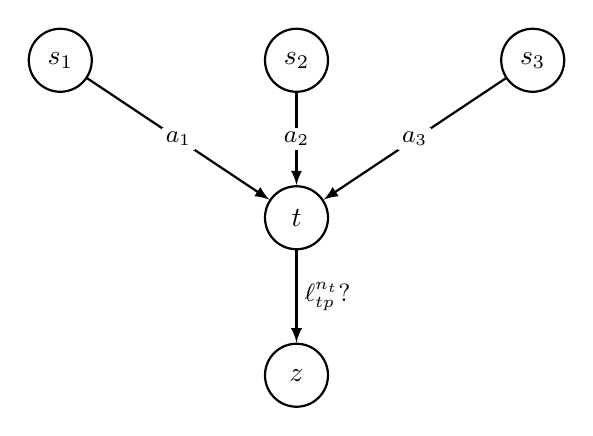
\begin{tikzpicture}[
            nd/.style={circle, draw, minimum size=8mm, inner sep=1pt},
            every edge/.style={draw, -latex, thick},
            lbl/.style={fill=white, inner sep=1.5pt, font=\small},
            thick
        ]
        \node[nd] (s1) at (0,3)   {$s_1$};
        \node[nd] (s2) at (3,3)   {$s_2$};
        \node[nd] (s3) at (6,3)   {$s_3$};
        \node[nd] (t)  at (3,1) {$t$};
        \node[nd] (z)  at (3,-1)   {$z$};
        \draw (s1) edge node[lbl] {$a_1$} (t);
        \draw (s2) edge node[lbl] {$a_2$} (t);
        \draw (s3) edge node[lbl] {$a_3$} (t);
        % \draw (t) edge node[lbl, right=1pt] {$\textstyle\sum_s a_s$} (z);
        \draw (t) edge node[lbl, right=1pt] {$\ell^{n_t}_{tp}$?} (z);
    \end{tikzpicture}
    \captionof{figure}{Toy model.
        Three sources draw $a_1,a_2,a_3$ into the single plant $t$, which delivers their sum to the single zone $z$.}
\end{center}

\noindent Since this is just the network model with routing fixed, going the other way needs nothing new: free the routing variables and add more sources, plants and zones.
The toy can therefore be built and tested first, then scaled up without reformulating.

\clearpage
\bibliographystyle{plainurl}
\bibliography{references}

\clearpage
\appendix
\section{Implicit constraints}\label{sec:implicit_constraints}

This appendix complements Section~\ref{sec:constraints} with inequalities that hold for the model but are not stated there explicitly.

\paragraph{Closed nodes send no flow.}
\begin{align}
    b_{st} & \le \overline{W}_s\,\alpha_s, \quad \forall s \in \mathcal{S},\ t \in \mathcal{T}, \label{eq:closed_source} \\
    c_{tz} & \le \overline{V}_t\,\beta_t, \quad \forall t \in \mathcal{T},\ z \in \mathcal{Z}. \label{eq:closed_plant}
\end{align}
By \eqref{eq:nonnegativity} and \eqref{eq:source_flow_conservation}, $b_{st} \le \sum_{t' \in \mathcal{T}} b_{st'} = a_s$, and $a_s \le \overline{W}_s\alpha_s$ by \eqref{eq:source_capacity}.
Likewise, \eqref{eq:nonnegativity} and \eqref{eq:plant_flow_conservation} give $c_{tz} \le \sum_{z' \in \mathcal{Z}} c_{tz'} = \sum_{s \in \mathcal{S}} b_{st}$, which is at most $\overline{V}_t\beta_t$ by \eqref{eq:plant_capacity}.
Hence a closed source or plant never sends water outwards.

\paragraph{Total supply covers total demand.}
Summing \eqref{eq:demand} over all zones and applying \eqref{eq:plant_flow_conservation}, \eqref{eq:source_flow_conservation} and \eqref{eq:source_capacity} gives
\begin{equation}\label{eq:total_supply}
    \sum_{s \in \mathcal{S}} \overline{W}_s\,\alpha_s
    \ \ge\ \sum_{s \in \mathcal{S}} a_s
    \ =\ \sum_{t \in \mathcal{T}} \sum_{z \in \mathcal{Z}} c_{tz}
    \ \ge\ \sum_{z \in \mathcal{Z}} D_z.
\end{equation}
Whatever the routing, the active sources must have enough combined capacity to cover total demand, so no set of sources whose maximum withdrawals sum to less than $\sum_z D_z$ can be the active set.

\paragraph{Blend bounds implied by outlet quality.}
Combining \eqref{eq:outlet_water_quality} with \eqref{eq:removal_process_initial} gives, for every $t \in \mathcal{T}$ and $p \in \mathcal{P}$:
\begin{align}
    \underline{Q}_p \sum_{s \in \mathcal{S}} b_{st}
     & \le \sum_{s \in \mathcal{S}} Q_{sp}\, b_{st}, \label{eq:implied_blend_lower}
\end{align}
This means the incapability of $t \in \mathcal T$ to correct a blend that is below a lower limit, assuming only removal process is implemented; thereby, every lower regulatory limit must be met by source selection and blending, $\forall p \in \mathcal P$.
Three cases follow.
\begin{itemize}
    \item If $\underline{Q}_p = 0$, \eqref{eq:implied_blend_lower} never binds, otherwise no water is drawn.
    \item If $\underline{Q}_p > 0$, as for alkalinity, \eqref{eq:implied_blend_lower} binds regardless of the processes installed at the plant.
    \item If no process acts on $p$ ($H_{trp} = 0$ for all $r \in \mathcal{R}_t$, or equivalently $e_{trp} = 0$, as for the transformed value \eqref{eq:ph_source_transformation}), then $\ell^{n_t}_{tp} = \ell^{0}_{tp}$ and
          \begin{equation*}
              \underline{Q}_p \sum_{s \in \mathcal{S}} b_{st}
              \le \sum_{s \in \mathcal{S}} Q_{sp}\, b_{st}
              \le \overline{Q}_p \sum_{s \in \mathcal{S}} b_{st},
          \end{equation*}
          so both limits must be met by blending alone.
\end{itemize}

\end{document}